%------------------------------------------------------------------------------
% Author(s):
% Varaun Ramgoolie
%
% Copyright:
%  Copyright (C) 2020 Brad Bachu, Arjun Mohammed, Varaun Ramgoolie, Nicholas Sammy
%
%  This file is part of Applied-Mathematics-Unit2 and is distributed under the
%  terms of the MIT License. See the LICENSE file for details.
%
%  Description:
%     Year: 2009
%     Module: 3
%     Question: 6
%------------------------------------------------------------------------------

%------------------------------------------------------------------------------
% 6 a
%------------------------------------------------------------------------------

\begin{subquestions}
	
\subquestion

\begin{subsubquestions}
	
\subsubquestion

\textbf{\textit{Sketch and Translate:}} \\ \\
\begin{figure}[H]
	\begin{center}
		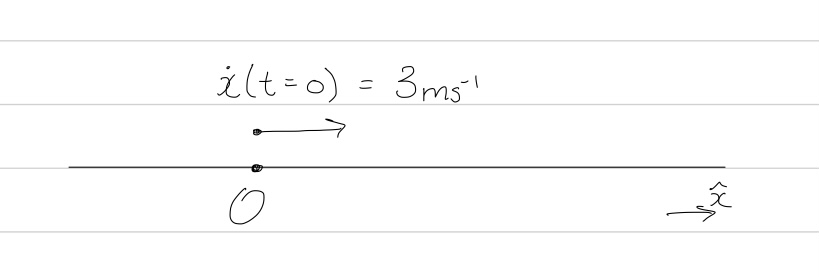
\includegraphics[scale=0.25]{../2009/figures/2009q6-1}
		\caption{\label{2009:q6:Sketch1} Movement of particle.}
	\end{center}
\end{figure}
We are given the acceleration as a function of time. At $t=0$, we know that the velocity, $v(t=0)$, is $3ms^{-1}$.
	
	
	
	
\textbf{\textit{Simplify and Diagram:}} \\ \\
\begin{figure}[H]
	\begin{center}
		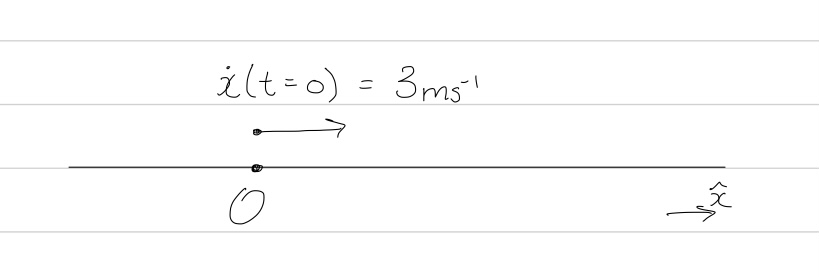
\includegraphics[scale=0.25]{../2009/figures/2009q6-1}
		\caption{\label{2009:q6:Diagram1} Movement of particle.}
	\end{center}
\end{figure}
As we are given the acceleration function, we can find the velocity function of the particle by integrating the given function between the appropriate bounds.




\textbf{\textit{Represent Mathematically:}} \\ \\
By definition, we know that,
\begin{align}
	a(t) & = \ddd{}{t}v(t) \nn \\
	\int_{t=0}^{t=t^\prime} a(t) dt &= v(t=t^\prime) - v(t=0) \\
	\implies \int_{t=0}^{t}a(t)\dd t & = \int_{v=3}^{v} \dd v(t) \nn \\
	\int_{t=0}^{t}a(t)\dd t & = v(t)-3 \label{2009:q6:VEqn1}
\end{align}
\TODO{Review integrals.}



\textbf{\textit{Solve and Evaluate:}} \\ \\
Solving \req{2009:q6:VEqn1}, we get that,
\begin{align}
	v(t')-3 & = \int_{t=0}^{t=t'}a(t)\dd t \nn \\
	     & = \int_{t=0}^{t=t'} 3t-9 \dd t \nn \\
	     & = \frac{3t'^2}{2}-9t' \nn \\
\implies v(t') & = \frac{3t'^2}{2}-9t' +3 \,.
\end{align}

Thus, substituting $t'=4$, we get that,
\begin{align}
	v(4) & = \frac{3(4)^2}{2}-9(4) +3 \nn \\
	     & = -9ms^{-1} \,.
\end{align}


%------------------------------------------------------------------------------

\subsubquestion

\textbf{\textit{Simplify and Diagram:}} \\ \\
We can use \rfig{2009:q6:Diagram1}. Similar to (a)(i), we can find the displacement function of the particle by integrating the velocity function between the appropriate bounds. At $t=0$, we will take $s$ to be $0$ as well




\textbf{\textit{Represent Mathematically:}} \\ \\
By definition, we know that,
\begin{align}
	v(t) & = \ddd{}{t}s(t) \nn \\
	\implies \int_{t=0}^{t}v(t)\dd t & = \int_{s=0}^{s} \dd s(t) \nn \\
	\int_{t=0}^{t}v(t)\dd t & = s(t)  \label{2009:q6:SEqn1}
\end{align}




\textbf{\textit{Solve and Evaluate:}} \\ \\
Solving \req{2009:q6:SEqn1}, we get that,
\begin{align}
	s(t') & = \int_{t=0}^{t=t'} v(t)\dd t \nn \\
	      & = \int_{t=0}^{t=t'} \frac{3t'^2}{2}-9t' +3 \dd t \nn \\
	      & = \frac{t'^3}{2} - \frac{9t'^2}{2} + 3t' \,.
\end{align}

Substituting $t'=4$, we get that,
\begin{align}
	s(4) & = \frac{4^3}{2} - \frac{9(4)^2}{2} + 3(4) \nn \\
	     & = -28m\,.
\end{align}
	
\end{subsubquestions}

%------------------------------------------------------------------------------
% 6 b
%------------------------------------------------------------------------------

\subquestion

Let us first define our positive direction as to the right of $O$. In (a)(i), our result means that the particle is moving at 9ms$^{-1}$ in the direction left of $O$\footnote{This is representative by the negative sign.}. In (a)(ii), our result tells us that the particle is 28m to the left of $O$.

%------------------------------------------------------------------------------
% 6 c
%------------------------------------------------------------------------------

\subquestion

\begin{subsubquestions}
	
\subsubquestion

\textbf{\textit{Sketch and Translate:}} \\ \\
\TODO{What diagram here?} We are given the position of a particle which is defined using time $t$. We can consider this as the displacement function of the particle with respect to time.




\textbf{\textit{Simplify and Diagram:}} \\ \\
As we are given the displacement function of the particle, in terms of the unit vectors $\ihat$ and $\jhat$, we can differentiate this twice to obtain the acceleration function of the particle.



 
\textbf{\textit{Represent Mathematically:}} \\ \\
By definition, we know that,
\begin{align}
	a(t) & = \ddd{}{t}v(t) \label{2009:q6:AEqn2} \,.
\end{align}

We also know,
\begin{align}
	v(t) & = \ddd{}{t}s(t) \label{2009:q6:VEqn2} \,.
\end{align}



\textbf{\textit{Solve and Evaluate:}} \\ \\
Firstly, we can use \req{2009:q6:VEqn2} to find,
\begin{align}
	v(t) & = \ddd{}{t}\left(8t\ihat + (t^4-32t)\jhat\right) \nn \\
	     & = 8\ihat + (4t^3-32)\jhat \,.
\end{align}

Now we can find the acceleration from \req{2009:q6:AEqn2} as,
\begin{align}
	a(t) & = \ddd{}{t}(8\ihat+(4t^3-32)\jhat) \nn \\
	     & = 0\ihat + (12t^2)\jhat \,.
\end{align}

As we have found that the coefficient of $\ihat$ in $a(t)$ is 0, we get that there is no acceleration in the direction of $\ihat$, which is along $Ox$. 

%------------------------------------------------------------------------------

\subsubquestion

\textbf{\textit{Simplify and Diagram:}} \\ \\
We have already found functions for velocity and acceleration. To find the time where both are perpendicular, we can take their dot product, set it to 0 and solve for $t$.




\textbf{\textit{Represent Mathematically:}} \\ \\
If $v(t)$ and $a(t)$ are perpendicular, we know that,
\begin{align}
	v(t) \cdot a(t) = 0 \label{2009:q6:DotEqn} \,.
\end{align}
\TODO{use full expression for dot product.}



\textbf{\textit{Solve and Evaluate:}} \\ \\
Using \req{2009:q6:DotEqn}, we find that the velocity and acceleration are perpendicular at,
\begin{align}
	v(t) \cdot a(t) & = 0 \nn \\
	\left(8\ihat + (4t^3-32)\jhat\right) \cdot \left(0\ihat + (12t^2)\jhat \right) & = 0 \nn \\
	\left(8 \times 0\right) + \left((4t^3-32) \times (12t^2)\right) & = 0 \nn \\
	12t^2\left(4t^3-32\right) & = 0 \nn \\
	\implies 12t^2 & = 0 \nn \\
	t & = 0 \\
	& \text{and,} \nn \\
	\implies 4t^3-32 & = 0 \nn \\
	t & = \sqrt[3]{8} = 2 \,.
\end{align}

\TODO{word the t=0 solution well.}

We should note, however, that the acceleration of the particle acts only along $Oy$ (from (c)(i)). Therefore, we could have also approached this problem by considering when the velocity of the particle acts \textbf{only} in along $Ox$ (as $Ox$ and $Oy$ are perpendicular).

%------------------------------------------------------------------------------

\subsubquestion

\textbf{\textit{Simplify and Diagram:}} \\ \\
As we are given the displacement function, we can find the magnitude of this function at $t=3$ to find the distance of the particle from O.




\textbf{\textit{Represent Mathematically:}} \\ \\
The distance away from O after time $t$ can be given as,
\begin{equation}
	\text{Distance} = |s(t)| \,.
\end{equation}




\textbf{\textit{Solve and Evaluate:}} \\ \\
At $t=3$, the distance from O is,
\begin{align}
	\text{Distance} & = |s(t)| \nn \\
	                & = |8(3)\ihat + (3^4-32(3))\jhat| \nn \\
	                & = |24\ihat + (-15)\jhat| \nn \\
	                & = \sqrt{(24^2)+(-15)^2} \nn \\
	                & = 28.3m
\end{align}




 
	
	
	
	
	
	
\end{subsubquestions}












	

	
	
	
\end{subquestions}









